\parindent 0in
\parskip 0.1in

{\bf Title:  Reduced Order Modeling of heat and fluid flow: Multi-scale
modeling of advanced reactors to enable faster deployment}

{\bf Technical work scope identification: M\&S 1 }

{\bf PI:}
Paul Fischer \\
Department of Computer Science \\
Department of Mechanical Science \& Engineering \\
University of Illinois, Urbana-Champaign \\

{\bf co-PIs:}
Elia Merzari, Pennsylvania State University, \\
Dillon Shaver, Argonne National Laboratory \\

\section{Project Summary}

% \begin{itemize}
% \item
% A summary of the proposed project, including a description of the project and a
% {\em clear explanation of its importance and relevance to the objectives in Part I
% Section A.}
% \item
% Major deliverables and outcomes the R\&D will produce.
% \item
% Timeframe of execution: October 1, 2023--September 30, 2026
% \end{itemize}

We seek \textbf{to develop novel multi-scale algorithmic approaches for the
simulation of heat and fluid flow in advanced reactors}. The methods, which
leverage recent advances in hardware and reduced order modeling approaches,
will enable fast-running simulations of vastly accelerated speed, while
maintaining accuracy comparable to high-fidelity methods such Large Eddy
Simulation (LES) and Direct Numerical Simulation (DNS). These methods will
allow to perform
parameter sweeps to assess uncertainty and develop closures. They will also
enable, for the first time, to perform high fidelity simulation of transients.

Several  advanced reactors concepts are currently being pursued in the United
States, with dozens of companies proposing unique designs. Crucial for their
deployment is the analysis of  reactor transients (e.g., a protected loss of
flow): an essential part of the evaluation of thermal margins and the overall
safety case.  In most cases, licensing will be pursued with established
methods, based on lumped parameter system codes (e.g., SAM \cite{hu2021}).
However, these codes require adequate closures that are typically obtained
empirically and require extensive validation. Furthermore, these methods are
characterized by high level of uncertainty when dealing with complex
three-dimensional turbulent flow, especially in the presence of large
enclosures, mixed convection, and thermal stratification. High-fidelity
simulation on the other hand remains prohibitively expensive, especially for
large parameter sweeps or for the simulation of nuclear transients, and data
remains sparse.

Moreover, as the advanced reactor industry matures and moves past demonstration
projects, economics will become a larger driver. This pressure will likely push
vendors to seek to maximize the economic potential (e.g., higher power output,
higher temperature for process heat, reduced capital cost), especially as new
materials and fuels are introduced. These goals will benefit from radically
improved methods to assess thermal margins that push toward high fidelity.
\textbf{This proposal seeks to develop radically novel algorithmic approaches
to the simulation of advanced reactors, with an unprecedented level of
fidelity, enabling transformative design approaches and improved economics.} 
In particular we aim to: 
\begin{enumerate}
%
   \item \textit{Enable the simulation of large parameter sweeps using reduced
   order models developed over a subset of the parameter space.} This approach
   will allow to assess uncertainty of system-level approaches and to develop
   closures.
%
   \item \textit{Enable the accelerated simulation of transients.}
   This approach will allow to assess lower resolution approaches in conjunction
   with experimental data for the simulation of transient.  
\end{enumerate}
As a demonstration application we choose the simulation of Sodium Fast Reactor
(SFR) fuel assemblies under steady-state and transient conditions. \textit{We
emphasize that the methods developed will apply to a broad range of advanced
reactor applications.}

\begin{figure}[t!] \centering
    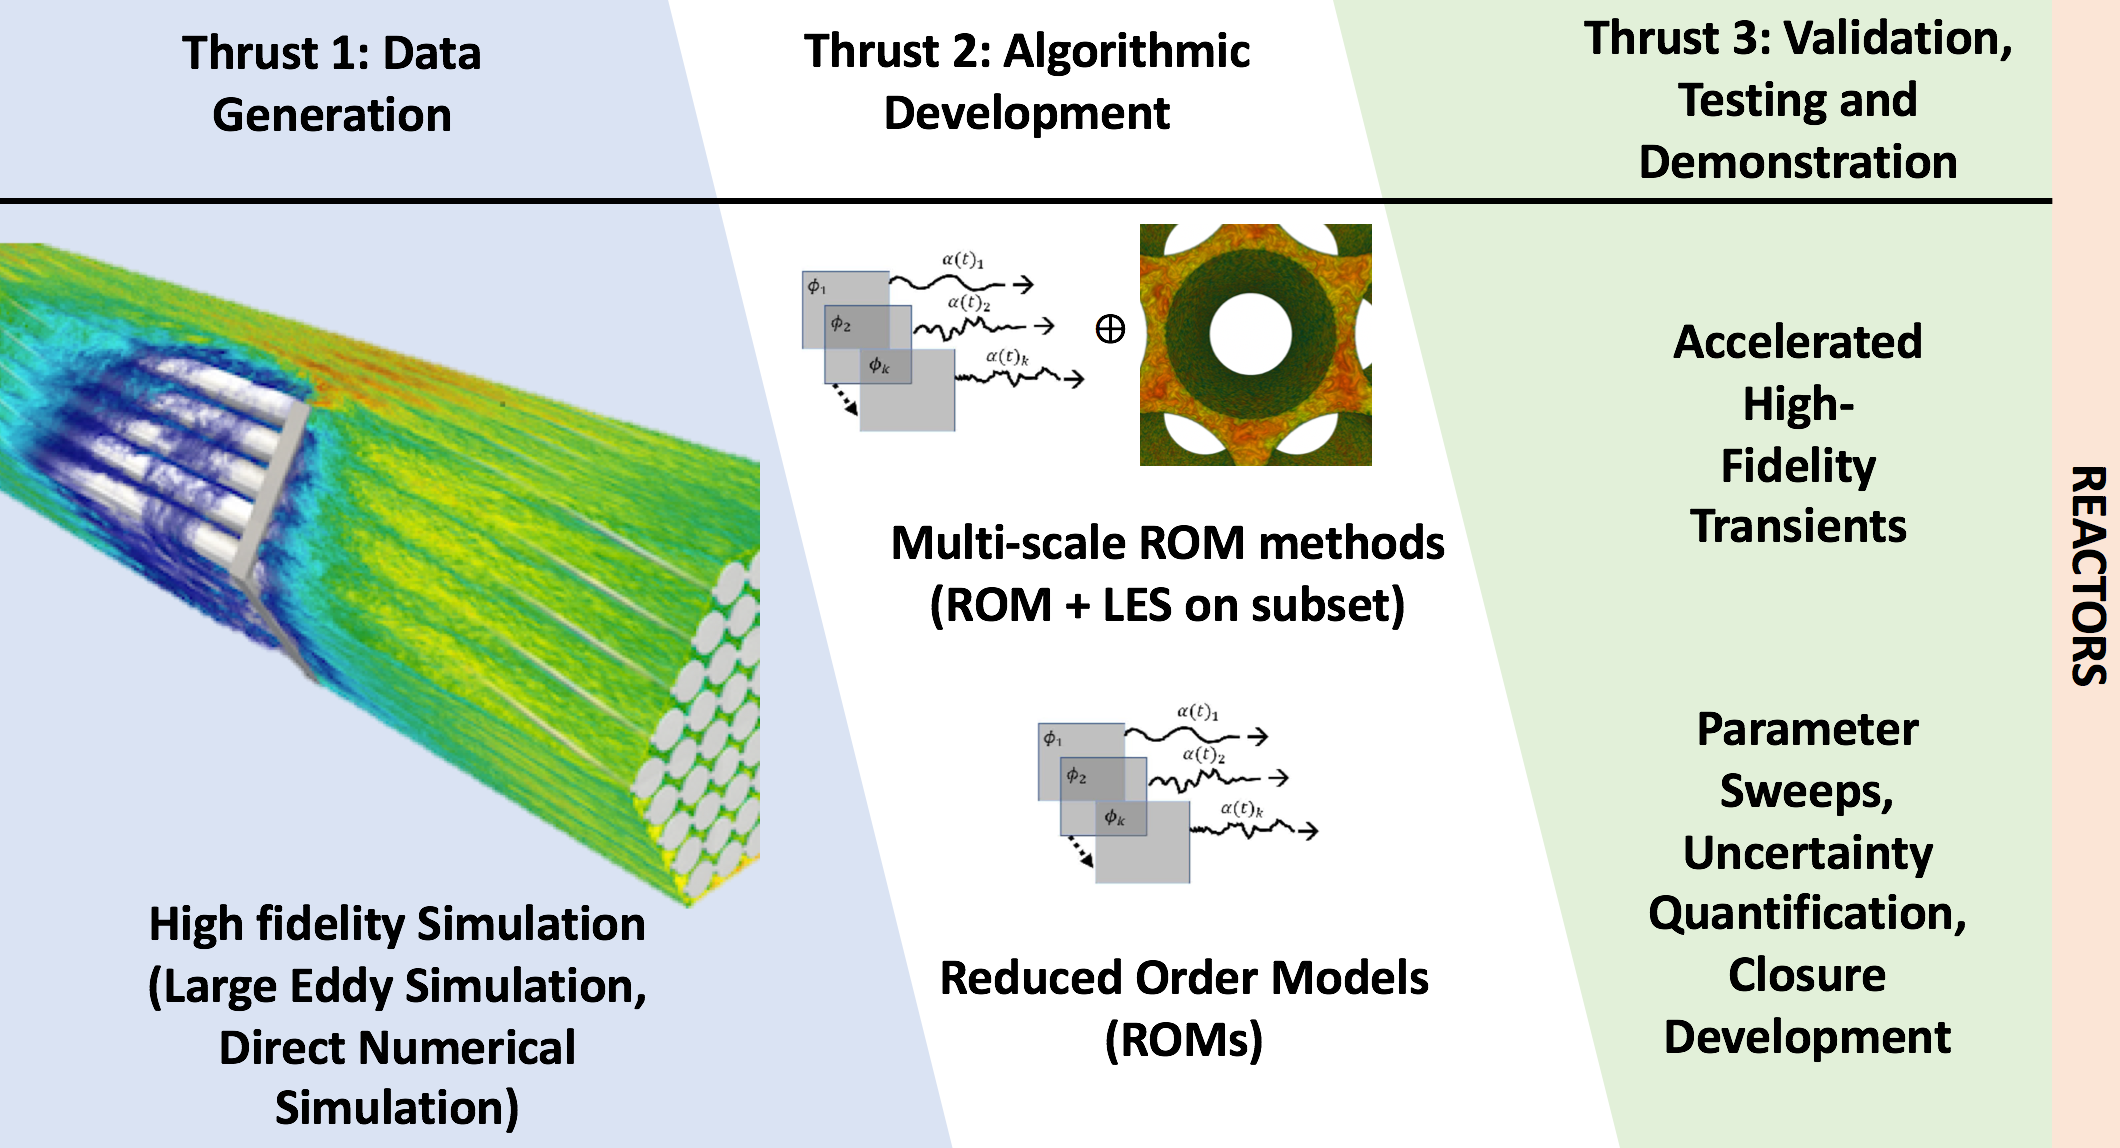
\includegraphics[width = 0.80\textwidth]{figs/overview.png}
    \caption{Overview of Project with three thrusts: Data generation,
             algorithmic development and validation/demonstration.  \label{fig:sum}}
\end{figure}


\section{Project Motivation and Technical Objectives}

We propose to leverage ongoing hardware, software, and algorithmic developments
to dramatically enhance thermal-hydraulic analysis capabilities.  The work will
entail combining advanced simulations on DOE's exascale computing platforms
with modern data analysis methods that effectively compress these
first-principle data to efficient exploratory tools based on reduced-order
models (ROMs).
We illustrate the project overview in Fig. \ref{fig:sum}.

\noindent
{\bf High-Fidelity Simulations on DOE Leadership Computers.}
The DOE is bringing several accelerator-based exascale platforms online,
including Frontier at ORNL and Aurora at ANL.
As illustrated in Fig. \ref{fig:pbr},
we have demonstrated that it is possible to simulate a single flow
through time for the thermal-hydraulics of a full pebble-bed reactor core
(352,000 pebbles) in just six hours of wall-clock time on ORNL's {\em
pre}-exascale machine, Summit.   This is an significant acheivement as it
involves updating a quarter-trillion degrees-of-freedom at $\approx$ 0.3
seconds per step.  
%This problem is relatively small for an exascale platform, on which it will be
%possible to explore multiple configurations in this space within an  annual
%allocation.  which will make it possible to consider parameter exploration
%that is critical for analysis and design.
The software that enables this achievement is {\em NekRS}, which is the
GPU-oriented version of the high-order spectral element code, Nek5000. 
NekRS is being developed under DOE's Center for Efficient Exascale Discretizations
(CEED) and sustains $\approx$ 0.5--1.0 TFLOPS ($10^{12}$ floating point
operations per second) per MPI rank on current pre-exascale platforms (e.g.,
Summit and Crusher at ORNL and Polaris at ANL).  It is a highly efficient code
that realizes 2--4 TFLOPS-FP64/rank on key kernels and 80\% parallel efficiency
with about 2M grid points per rank.  Consequently, a 50B grid-point problem
such as the full pebble-bed reactor core of Fig. \ref{fig:pbr} can effectively
use $P$=25,000 GPUs (or GCDs in the case of Frontier or tiles in the case of
Aurora).  While such a calculation essentially fills all of Summit, it would
use only a fraction of Frontier or Aurora.  On these platforms, we can
anticipate running larger problems or running at multiple points in the reactor
design space.  Execution times on these platforms can be anticipated to remain
at $\approx$ 0.1--0.3 seconds per step, even with larger problems running on
the full systems.



\begin{figure}[t!] \centering
    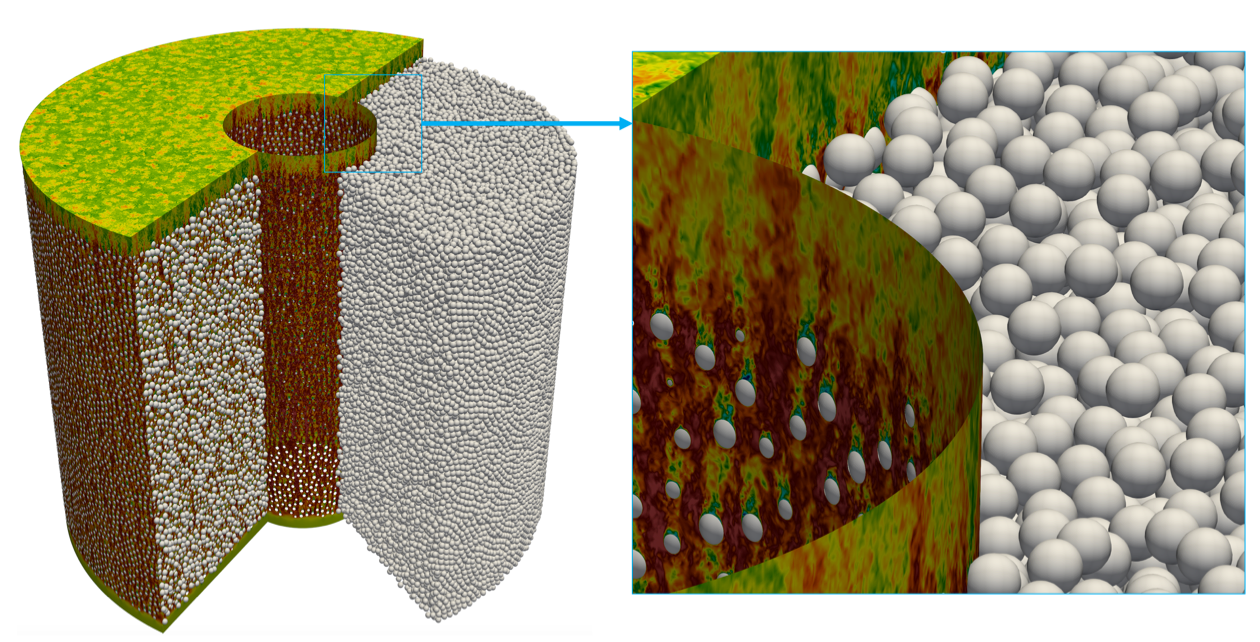
\includegraphics[width = 0.60\textwidth]{figs/pbr_pair.png}
    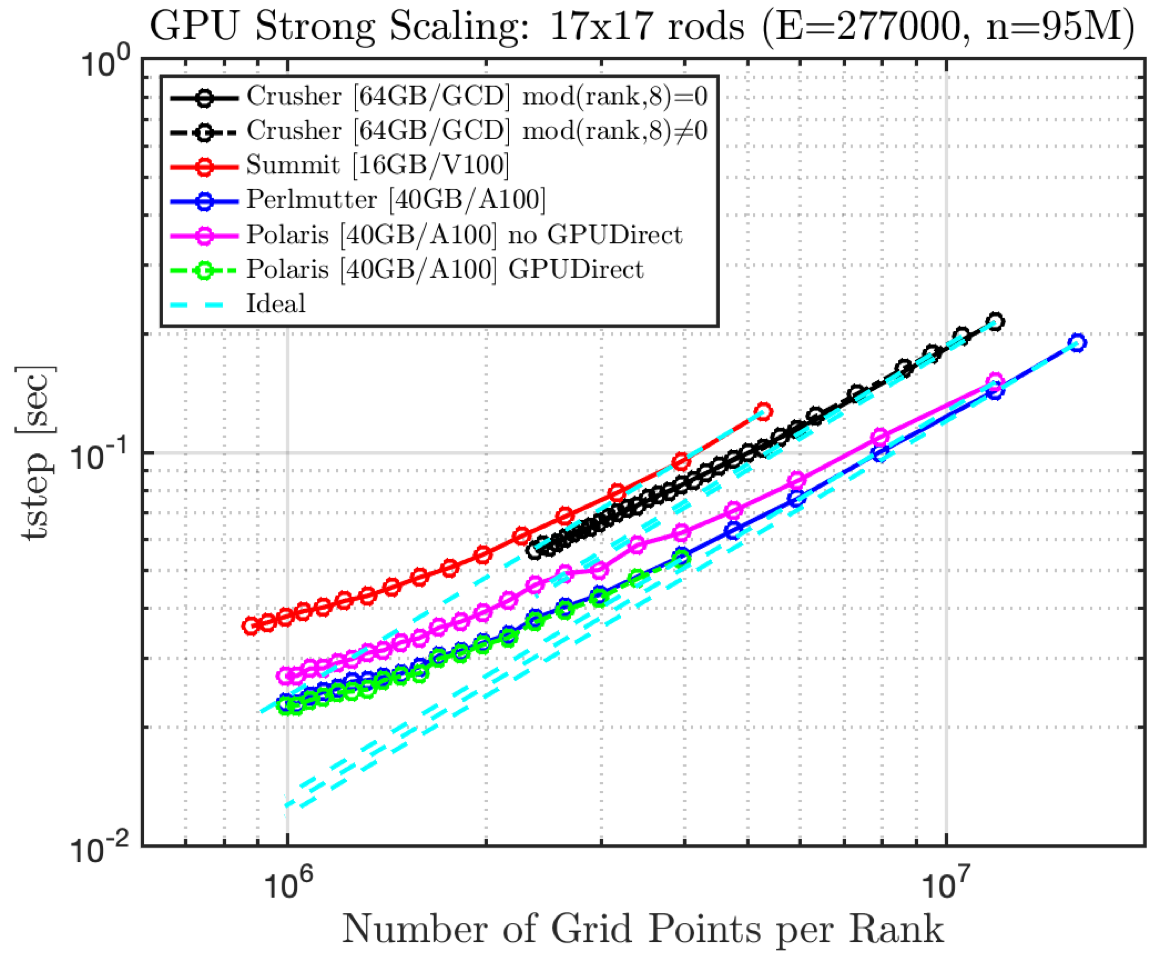
\includegraphics[width = 0.35\textwidth]{figs/nekrs_17x17_crusher_strong.png}
    \caption{(left) NekRS turbulent flow simulation results for a full reactor
core with 352625 pebbles.  The simulation comprised 51 billion gridpoints
($E$=99M spectral elements of order $p$=8).  On all of Summit (27648 NVIDIA
V100 GPUs), this simulation requires 0.36 seconds per step and would complete a
single flow-through time in just six hours. (Computation by Yu-Hsiang Lan,
ANL/UIUC.)
(right) NekRS strong-scaling on current-generation accelerator-based platforms:
AMD-MI250X-based Crusher (OLCF),
NVIDIA-V100-based Summit (OLCF),
NVIDIA-A100-based Perlmutter (NERSC),
NVIDIA-A100-based Polaris (ALCF).
The test problem is a 17$\times$17 rod-bundle with 95 million grid points.
(Simulations by Misun Min, ANL, and Yu-Hsiang Lan, ANL/UIUC.)
\label{fig:pbr}}
\end{figure}


%% (WHY ROM)
\noindent
{\bf Data-Driven Reduced-Order Models.}
While it is clear that NekRS will be capable of delivering fast turn-around
for reactor-scale simulations on DOE's exascale platforms, the use of 
such simulations for one-off determination of system behavior at a single
parameter point does not fully leverage the data generated by such a large
calculation.
From a design perspective, it would be far more efficient if one could reliably
explore parametric input/output relationships (e.g., Nusselt/Rayleigh-number
relationships under low-flow conditions) in the neighborhood of the parameter
space for which the high-fidelity DNS or LES is performed.   Such a capability
is precisely the goal of parametric model-order reduction (pMOR), which is
typically based on reduced-order models (ROMs) of the high-fidelity DNS/LES
(often referred to as full-order models, or FOMs).   

Under NEUP Award 18-15520 we have developed have developed a pMOR/ROM
capability withing the Nek5000 framework that allows users to build ROMs and
perform parameter variation with these models.  The development of ROMs for
unsteady (e.g., turbulent or transient) flows is still an open research topic.
In broad terms, the process consists of two problems: {\em (i) the solution
reproduction problem}, and {\em (ii) the parametric problem}.  To these, we add
a third category that of interest to the current project: {\em (iii) evolution
of long transients}.

We begin with the reproduction problem. The standard approach is to use
$\approx 1000$ high-fidelity solution snapshots (i.e., full velocity/temperature
fields) to extract $N$$\approx$20--200 basis functions through 
proper-orthogonal decomposition (POD) or some other low-rank approximation
approach.  Using these basis functions one can construct a low-rank
dynamical system from the governing Navier-Stokes and energy-transport
equations that governs the unknown basis coefficients.  These systems,
which are of size $N$, run extremely fast---on a laptop, it is possible
to evolve tens-of-thousands of convective time units in a minute, far more than
is feasible with the FOM, which is one of the reasons that ROMs are interesting
for long-time transients.  Moreover, it is relatively easy to adjust equation
parameters to have a nominal pMOR tool.  (Adjusting geometry is more
challenging and one of the topics to be explored in the context of this
project).

There are several challenges to bring the preceding scenario to fruition.
The first is to ensure that the ROM can effectively track the quantities
of interest (QOIs) produced by the FOM, even at the same parameter point.
This tracking is by no means assured, particularly for turbulent flows
where energy is dissipated by small-scale structures that are generally
absent from POD bases.  Several stabilization strategies are possible,
such as 












, the development of ROM








NekROM, which is a software
too

uuuu


%\section{Project Narrative}
%% Applicant shall provide a written narrative addressing the strategy
%% to execute R&D that supports the specified Technical Workscope. The
%% documentation provided shall include the items specified below:

\vspace*{.0in} \noindent 
\underline{\textbf{Title of Project}} 
\\[-2ex]

\noindent
\textbf{Multiscale Modeling for Reactor Thermal Hydraulics}


\vspace*{.15in} \noindent 
\underline{\textbf{Technical Workscope Identification:  NEAMS-1.4}}
\\[-2ex]


\vspace*{.05in} \noindent 
\underline{\textbf{Project Objectives.}} 
\\[-2ex]

  The objective of this project is to develop a reduced-order model for the
simulation of stratified flows characteristic of the upper plenum in liquid
metal reactors.  The code suite will translate high-fidelity large-eddy
simulations of turbulent stratified flow into a set of coefficients that can
drive a low-dimensional dynamical system relating output to input quantities
(e.g., temperatures and flow rates in a multiport plenum) suitable for 
systems analysis codes.  
\\[0ex]

\vspace*{.0in}\noindent \underline{\textbf{Proposed Scope Description}}%  (< 1 page )
\\[-2ex]


The scope of the proposed work is to develop an effective {\em analysis chain}
that will allow designers to accurately predict thermal-hydraulics behavior
over the broad range of temporal and spatial scales that are relevant to overall
reactor behavior.
    The tools to tackle this multiscale phenomena include NekRS, which is 
a GPU-variant of Nek5000 that is designed to fully leverage the performance of
DOE's leadership computers, including the exascale platforms Frontier and
Aurora; and NekROM, which is a new reduced-order modeling module within
Nek5000/RS that was developed under NEUP Award 18-15520.






{\em reduced-order
models} (ROMs) for reactor thermal design and analysis with the specific target
problem of the upper plenum in a liquid metal reactor (LMR).  Characteristics
of flow in the upper plenum include multiple inlets at various temperatures, a
stratified background, natural circulation, and multiple outlets.  
   ROMs typically comprise a small system of ordinary differential equations
(ODEs) that represent the evoluton of $N \approx 100$ basis functions designed
to capture the dominant dynamics of the flow field.
   {\em Parametric model order reduction} (pMOR) is a process through which
a ROM or suite of ROMs is constructed to estimate the system behavior 
over a range of parametric inputs (e.g., inlet flow rates, Reynolds number)
without the need for high-fidelity simulations at every point in the target
parameter space.  The output of the pMOR will be a small set 
of coefficients to drive low-rank systems of ODEs that can be directly coupled
with into the Aystems Analysis Module (SAM) to provide a more accurate response
than currently-used zero-dimensional models for the upper plenum.

The ROMs will be derived from high-fidelity direct numerical
(DNS), large-eddy (LES), or unsteady Reynolds-averaged Navier-Stokes (uRANS)
simulations of turbulent thermal transport, which will performed on DOE's
leadership computing facilities in an {\em offline} mode using the
NEAMS-supported Nek5000 code.  The ROMs will be used in a real-time {\em
online} mode (e.g., in SAM), simulating the governing Navier-Stokes and energy
equations as a projection of a small set of basis functions derived from a
proper-orthogonal-decomposition (POD) of snapshots generated by the
high-fidelity simulations.  Innovative features of the proposed work include a
stabilized POD-Galerkin formulation based on constrained optimization,
efficient algorithms for basis selection to minimize the size, $N$, of the
reduced basis set;  and a rapidly convergent greedy training scheme using
dual-norm based error indicators to provide accurate analyses at low cost.  
Verification and validation (V\&V) will be performed by comparing the ROM
against DNS/LES-based full-order models (FOM) {\em and} against available
experimental data relevant to the upper plenum (e.g., \cite{lomperski17}).


The proposed analysis tool requires 
 \textbf{i.} detailed full-order simulations of size (number of degrees-of-freedom)
$\cN=10^7$--$10^{11}$;
 \textbf{ii.} a software module within Nek5000 to distill each full-order
simulation into ROMs of size $N \approx 100$;
 \textbf{iii.} a software driver to iterate between the ROM and Nek5000 to 
pick optimal anchor (trial) points in the target parameter 
(e.g., Reynolds or Prandtl number) space, $\cP$;
and
 \textbf{iv.} a simulation code to evolve the ROM in the online mode. 
The principal focus will be on developing ( \textbf{ii.}-- \textbf{iv.}), supported by
simulations with Nek5000 (\textbf{i.}), which is well-established as a scalable
code for solving the full-order models (e.g., \cite{merzari11b,merzari15a}). 

Realization of a viable analysis tool requires economization of costs at all
stages of the process, including a reduction in the number of expensive
offline simulations and a reduction in the size of the
reduced-basis sets $N$, which incur costs scaling as $O(N^3)$ because 
of the nonlinear interactions in the Navier-Stokes equations.
In addition to costs, stability and accuracy of the ROM are also critical.

  To address these concerns, the proposed methodology will expand upon recent
developments in ROMs for long-time simulations of turbulent flows outlined in
\cite{fick18}.  Key ingredients of this approach are:
 \textbf{i.} $H^1_0$-POD-based basis sets for unsteady turbulent flows
         at fixed anchor points $\cP_{\mbox{\tiny anch}}$ in the target
         parameter space, $\cP$;
 \textbf{ii.} a novel constraint-based stabilization of the ROM derived
          from the full-order models;
 \textbf{iii.} effective dual-norm error estimates that {\em inexpensively}
           indicate the model error at any point in $\cP$; and
 \textbf{iv.} an efficient greedy algorithm for optimizing the choice of
          anchor points to meet the desired model error tolerance 
          for any point $\up^* \in \cP$.
We remark that the error estimators are essential to an efficient POD
formulation of this problem and are a {\em unique} contribution of the proposed
approach.  The constraint-based stabilization of the ROM is also {\em unique}
to the proposed effort.  This project will provide the first tests of this
approach in industrially-relevant settings.   

\vspace*{.08in}\noindent \underline{\textbf{ Logical Path to Accomplishing Scope.}} \\[-2ex]

As part of the development effort, the project will address several NE-relevant
test cases for validation of the overall modeling process.  We will start by
extending the 2D unsteady lid-driven cavity problem of \cite{fick18} to support
the energy equations.  We will next consider forced turbulent convection in a
T-junction, for which significant Nek5000 simulation and POD models have
already been validated against experimental data \cite{merzari11b}.
The final extension to address buoyancy-driven flows, such as arise in
the upper plenum
of Liquid Metal Reactors (LMRs) \cite{mbd1,mbd2,mbd3} based on available test data
as in \cite{mbd4} and prepare an input for system analysis modules (SAMs).  This
effort will include careful setup and validation of the full-order Nek5000 models 
for the target upper plenum simulations and identification of relevant 
upper plenum QOI's needed for the Systems Analysis Module.
\\[-1ex]



The proposed work has been broken into four tasks to be carried
out over the three-year project period: \\[-4.0ex]
\begin{itemize}
\item Task 1:  Extension of \cite{fick18} to 3D turbulent flows.
\\[-4.3ex]
\item Task 2:  Extension to the energy equation and thermally-driven QOIs.
\\[-4.3ex]
\item Task 3:  3D turbulent flows with thermal transport.
\\[-4.3ex]
\item Task 4:  Extension to buoyant 3D turbulent flows.
\end{itemize}
Task 1 is a logical first extension to the methodology described in \cite{fick18},
which used the unsteady 2D lid-driven cavity as a test problem.  
Task 2 incorporates an additional equation and thus requires additional
theory to establish appropriate error indicators for QOIs relevant to thermal
transport.
Task 3 combines the results from Tasks 1 and 2 for a first trial of
the method for turbulent thermal transport.
Task 4 incorporates additional (linear) coupling in the ROM methodology.

Each Task $\tau$ has the following subtasks, \\[-4ex]
\begin{itemize}
\item %Task $\tau$:
%\\[-3.6ex]
   \begin{itemize}
     \item Subtask $\tau$.1: Set up/execute DNS/LES full-order model in Nek5000
\\[-3.6ex]
     \item Subtask $\tau$.2: Formulation of error indicators for the problem.
\\[-3.6ex]
     \item Subtask $\tau$.3: Identify POD requirements (e.g., number of input
                       snapshots and size of the POD basis) for the
                       {\em solution reproduction problem}.
\\[-3.6ex]
     \item Subtask $\tau$.4: Build/extend the offline/online ROM 
                       modules to accommodate the new physics.
\\[-3.6ex]
     \item Subtask $\tau$.5: Verification/validation tests for the {\em parametric problem}. \\[-4ex]
   \end{itemize}
\end{itemize}
We note that verification/validation ($\tau$.5) is relatively straightforward in
the ROM setting given that one can run a full-order model at any test point in
a valid parameter range $\cP$.  Moreover, the sequence of Tasks,
$\tau$=$1,\dots,4$ is part of the validation process.  Each Task is an incremental
step between the current state of the art of 2D unsteady ``turbulence'' to the
target of 3D buoyancy-driven turbulence.  This systematic approach allows 
identification of potential pitfalls along the development path.

The effort requires correct problem specifications (parameters, boundary
conditions, mesh resolution, etc.) and efficient set-up of the large-scale
full-order models (FOMs) on DOE's leadership computing facilities.  We
anticipate acquiring computer time through DOE's standard award mechanisms
(director's discretionary, ALCC, or INCITE) and leveraging other resources
already available to the team members.  The ROM-modeling will involve extension
of the 2D unsteady Navier-Stokes setting in \cite{fick18} to 3D turbulent flows
with energy transport.  The error estimators will be modified to account for
quantities of interest (QOIs) relevant to the upper plenum flow, such as mean
and RMS temperature distributions, mean outflow distributions, etc.
Insight to temporal behavior will also be accessible from visualizations
of the ROM reconstructions.

\input narrative/plan

\input narrative/rom

\input narrative/merit

\vspace*{.05in}\noindent \underline{\textbf{Relevance and Outcomes/Impacts}} \\[-2ex]
\input narrative/relevance

%% • Relevance and Outcomes/Impacts: This section will explain the 
%%   program relevance/priority of the effort to the objectives in the 
%%   program announcement and the expected outcomes and/or impacts.


\vspace*{.05in}\noindent \underline{\textbf{Schedule}} \\[-2ex]
\input narrative/schedule 

\vspace*{.05in}\noindent \underline{\textbf{Milestones and Deliverables}} \\[-2ex]
\input narrative/milestones 

\vspace*{.05in}\noindent \underline{\textbf{Facilities}}
% • Type/Description of facilities that will be used to execute the
%   scope (if applicable).

\input narrative/facilities

\vspace*{.05in}\noindent \underline{\textbf{Roles/Responsibilities of 
Partnering Organizations}}

\input narrative/coordination


\vspace*{.05in}\noindent \underline{\textbf{Unique Challenges}}
% Unique challenges to accomplishing the work and planned mitigations.

\input narrative/challenge


